\documentclass{article}\usepackage[]{graphicx}\usepackage[]{color}
% maxwidth is the original width if it is less than linewidth
% otherwise use linewidth (to make sure the graphics do not exceed the margin)
\makeatletter
\def\maxwidth{ %
  \ifdim\Gin@nat@width>\linewidth
    \linewidth
  \else
    \Gin@nat@width
  \fi
}
\makeatother

\definecolor{fgcolor}{rgb}{0.345, 0.345, 0.345}
\newcommand{\hlnum}[1]{\textcolor[rgb]{0.686,0.059,0.569}{#1}}%
\newcommand{\hlstr}[1]{\textcolor[rgb]{0.192,0.494,0.8}{#1}}%
\newcommand{\hlcom}[1]{\textcolor[rgb]{0.678,0.584,0.686}{\textit{#1}}}%
\newcommand{\hlopt}[1]{\textcolor[rgb]{0,0,0}{#1}}%
\newcommand{\hlstd}[1]{\textcolor[rgb]{0.345,0.345,0.345}{#1}}%
\newcommand{\hlkwa}[1]{\textcolor[rgb]{0.161,0.373,0.58}{\textbf{#1}}}%
\newcommand{\hlkwb}[1]{\textcolor[rgb]{0.69,0.353,0.396}{#1}}%
\newcommand{\hlkwc}[1]{\textcolor[rgb]{0.333,0.667,0.333}{#1}}%
\newcommand{\hlkwd}[1]{\textcolor[rgb]{0.737,0.353,0.396}{\textbf{#1}}}%
\let\hlipl\hlkwb

\usepackage{framed}
\makeatletter
\newenvironment{kframe}{%
 \def\at@end@of@kframe{}%
 \ifinner\ifhmode%
  \def\at@end@of@kframe{\end{minipage}}%
  \begin{minipage}{\columnwidth}%
 \fi\fi%
 \def\FrameCommand##1{\hskip\@totalleftmargin \hskip-\fboxsep
 \colorbox{shadecolor}{##1}\hskip-\fboxsep
     % There is no \\@totalrightmargin, so:
     \hskip-\linewidth \hskip-\@totalleftmargin \hskip\columnwidth}%
 \MakeFramed {\advance\hsize-\width
   \@totalleftmargin\z@ \linewidth\hsize
   \@setminipage}}%
 {\par\unskip\endMakeFramed%
 \at@end@of@kframe}
\makeatother

\definecolor{shadecolor}{rgb}{.97, .97, .97}
\definecolor{messagecolor}{rgb}{0, 0, 0}
\definecolor{warningcolor}{rgb}{1, 0, 1}
\definecolor{errorcolor}{rgb}{1, 0, 0}
\newenvironment{knitrout}{}{} % an empty environment to be redefined in TeX

\usepackage{alltt}
\usepackage[top=1in,bottom=1in,left=1in,right=1in]{geometry}

\usepackage{setspace}

\usepackage{hyperref}
\hypersetup{colorlinks=true, urlcolor=blue, breaklinks=true}

\newcommand{\link}[1]{\footnote{\color{blue}\href{#1}{#1}}}
\newcommand{\myhref}[1]{\href{#1}{#1}}

\usepackage{amsmath}
\usepackage{amssymb}
\usepackage{mathtools}
\usepackage{linguex}
\usepackage{natbib}

%\usepackage{Sweave}





% The package for linguistics examples

\title{Plot and examine chains: 6 regions (no wrap-up; no matrix verb)}
\author{JD}
\IfFileExists{upquote.sty}{\usepackage{upquote}}{}
\begin{document}

\maketitle

\section{Simple model and plots}

This file collects draws and generates plots and info about parameters.

\begin{knitrout}
\definecolor{shadecolor}{rgb}{0.969, 0.969, 0.969}\color{fgcolor}\begin{kframe}
\begin{alltt}
\hlstd{burnin} \hlkwb{<-} \hlnum{500}

\hlkwd{library}\hlstd{(DBI)}
\hlkwd{library}\hlstd{(dplyr)}
\end{alltt}


{\ttfamily\noindent\itshape\color{messagecolor}{\#\# \\\#\# Attaching package: 'dplyr'}}

{\ttfamily\noindent\itshape\color{messagecolor}{\#\# The following objects are masked from 'package:stats':\\\#\# \\\#\#\ \ \ \  filter, lag}}

{\ttfamily\noindent\itshape\color{messagecolor}{\#\# The following objects are masked from 'package:base':\\\#\# \\\#\#\ \ \ \  intersect, setdiff, setequal, union}}\begin{alltt}
\hlkwd{library}\hlstd{(rstan)}
\end{alltt}


{\ttfamily\noindent\itshape\color{messagecolor}{\#\# Loading required package: StanHeaders}}

{\ttfamily\noindent\itshape\color{messagecolor}{\#\# Loading required package: ggplot2}}

{\ttfamily\noindent\itshape\color{messagecolor}{\#\# rstan (Version 2.21.1, GitRev: 2e1f913d3ca3)}}

{\ttfamily\noindent\itshape\color{messagecolor}{\#\# For execution on a local, multicore CPU with excess RAM we recommend calling\\\#\# options(mc.cores = parallel::detectCores()).\\\#\# To avoid recompilation of unchanged Stan programs, we recommend calling\\\#\# rstan\_options(auto\_write = TRUE)}}\begin{alltt}
\hlkwd{library}\hlstd{(loo)}
\end{alltt}


{\ttfamily\noindent\itshape\color{messagecolor}{\#\# This is loo version 2.3.1}}

{\ttfamily\noindent\itshape\color{messagecolor}{\#\# - Online documentation and vignettes at mc-stan.org/loo}}

{\ttfamily\noindent\itshape\color{messagecolor}{\#\# - As of v2.0.0 loo defaults to 1 core but we recommend using as many as possible. Use the 'cores' argument or set options(mc.cores = NUM\_CORES) for an entire session.}}

{\ttfamily\noindent\itshape\color{messagecolor}{\#\# \\\#\# Attaching package: 'loo'}}

{\ttfamily\noindent\itshape\color{messagecolor}{\#\# The following object is masked from 'package:rstan':\\\#\# \\\#\#\ \ \ \  loo}}\begin{alltt}
\hlstd{c1} \hlkwb{<-} \hlkwd{read.csv}\hlstd{(}\hlstr{"chain1/chain-0.csv"}\hlstd{)}

\hlstd{dataf} \hlkwb{<-} \hlkwd{select}\hlstd{(c1,} \hlkwd{starts_with}\hlstd{(}\hlstr{"subj_mu_rt"}\hlstd{))}

\hlstd{dataf}\hlopt{$}\hlstd{std} \hlkwb{<-} \hlstd{c1}\hlopt{$}\hlstd{std}

\hlstd{dataf} \hlkwb{<-} \hlstd{dataf[burnin}\hlopt{:}\hlkwd{length}\hlstd{(dataf[,} \hlnum{1}\hlstd{]), ]}

\hlkwd{str}\hlstd{(dataf)}
\end{alltt}
\begin{verbatim}
## 'data.frame':	5009 obs. of  7 variables:
##  $ subj_mu_rt__0: num  350 350 350 350 350 ...
##  $ subj_mu_rt__1: num  348 348 345 345 347 ...
##  $ subj_mu_rt__2: num  311 311 311 311 311 ...
##  $ subj_mu_rt__3: num  385 385 379 379 384 ...
##  $ subj_mu_rt__4: num  337 337 337 337 337 ...
##  $ subj_mu_rt__5: num  311 311 311 311 311 ...
##  $ std          : num  34.9 34.9 34.9 29.3 26.9 ...
\end{verbatim}
\begin{alltt}
\hlstd{dataf2} \hlkwb{<-} \hlkwd{select}\hlstd{(c1,} \hlkwd{starts_with}\hlstd{(}\hlstr{"obj_mu_rt"}\hlstd{))}

\hlstd{dataf2}\hlopt{$}\hlstd{std} \hlkwb{<-} \hlstd{c1}\hlopt{$}\hlstd{std}

\hlstd{dataf2} \hlkwb{<-} \hlstd{dataf2[burnin}\hlopt{:}\hlkwd{length}\hlstd{(dataf2[,} \hlnum{1}\hlstd{]), ]}

\hlkwd{str}\hlstd{(dataf2)}
\end{alltt}
\begin{verbatim}
## 'data.frame':	5009 obs. of  7 variables:
##  $ obj_mu_rt__0: num  350 350 350 350 350 ...
##  $ obj_mu_rt__1: num  345 345 345 345 345 ...
##  $ obj_mu_rt__2: num  385 385 379 379 384 ...
##  $ obj_mu_rt__3: num  378 382 379 376 380 ...
##  $ obj_mu_rt__4: num  348 349 349 348 349 ...
##  $ obj_mu_rt__5: num  311 311 311 311 311 ...
##  $ std         : num  34.9 34.9 34.9 29.3 26.9 ...
\end{verbatim}
\begin{alltt}
\hlstd{c2} \hlkwb{<-} \hlkwd{read.csv}\hlstd{(}\hlstr{"chain2/chain-0.csv"}\hlstd{)}

\hlstd{dataf.c2} \hlkwb{<-} \hlkwd{select}\hlstd{(c2,} \hlkwd{starts_with}\hlstd{(}\hlstr{"subj_mu_rt"}\hlstd{))}

\hlstd{dataf.c2}\hlopt{$}\hlstd{std} \hlkwb{<-} \hlstd{c2}\hlopt{$}\hlstd{std}

\hlstd{dataf.c2} \hlkwb{<-} \hlstd{dataf.c2[burnin}\hlopt{:}\hlkwd{length}\hlstd{(dataf.c2[,} \hlnum{1}\hlstd{]), ]}

\hlstd{dataf} \hlkwb{<-} \hlkwd{rbind}\hlstd{(dataf, dataf.c2)}

\hlkwd{str}\hlstd{(dataf)}
\end{alltt}
\begin{verbatim}
## 'data.frame':	10018 obs. of  7 variables:
##  $ subj_mu_rt__0: num  350 350 350 350 350 ...
##  $ subj_mu_rt__1: num  348 348 345 345 347 ...
##  $ subj_mu_rt__2: num  311 311 311 311 311 ...
##  $ subj_mu_rt__3: num  385 385 379 379 384 ...
##  $ subj_mu_rt__4: num  337 337 337 337 337 ...
##  $ subj_mu_rt__5: num  311 311 311 311 311 ...
##  $ std          : num  34.9 34.9 34.9 29.3 26.9 ...
\end{verbatim}
\begin{alltt}
\hlstd{dataf2.c2} \hlkwb{<-} \hlkwd{select}\hlstd{(c2,} \hlkwd{starts_with}\hlstd{(}\hlstr{"obj_mu_rt"}\hlstd{))}

\hlstd{dataf2.c2}\hlopt{$}\hlstd{std} \hlkwb{<-} \hlstd{c2}\hlopt{$}\hlstd{std}

\hlstd{dataf2.c2} \hlkwb{<-} \hlstd{dataf2.c2[burnin}\hlopt{:}\hlkwd{length}\hlstd{(dataf2.c2[,} \hlnum{1}\hlstd{]), ]}

\hlstd{dataf2} \hlkwb{<-} \hlkwd{rbind}\hlstd{(dataf2, dataf2.c2)}

\hlkwd{str}\hlstd{(dataf2)}
\end{alltt}
\begin{verbatim}
## 'data.frame':	10018 obs. of  7 variables:
##  $ obj_mu_rt__0: num  350 350 350 350 350 ...
##  $ obj_mu_rt__1: num  345 345 345 345 345 ...
##  $ obj_mu_rt__2: num  385 385 379 379 384 ...
##  $ obj_mu_rt__3: num  378 382 379 376 380 ...
##  $ obj_mu_rt__4: num  348 349 349 348 349 ...
##  $ obj_mu_rt__5: num  311 311 311 311 311 ...
##  $ std         : num  34.9 34.9 34.9 29.3 26.9 ...
\end{verbatim}
\begin{alltt}
\hlstd{ndraws} \hlkwb{<-} \hlkwd{length}\hlstd{(dataf2[,} \hlnum{1}\hlstd{])}

\hlstd{data.all} \hlkwb{<-} \hlkwd{data.frame}\hlstd{(}\hlkwc{word_no} \hlstd{=} \hlkwd{rep.int}\hlstd{(}\hlkwd{rep}\hlstd{(}\hlkwd{paste}\hlstd{(}\hlstr{"No"}\hlstd{,} \hlnum{3}\hlopt{:}\hlnum{8}\hlstd{,} \hlkwc{sep} \hlstd{=} \hlstr{""}\hlstd{),} \hlkwc{each} \hlstd{= ndraws),}
    \hlnum{2}\hlstd{),} \hlkwc{word} \hlstd{=} \hlkwd{factor}\hlstd{(}\hlkwd{rep}\hlstd{(}\hlkwd{rep}\hlstd{(}\hlkwd{c}\hlstd{(}\hlstr{"who"}\hlstd{,} \hlstr{"sent /\textbackslash{}nthe"}\hlstd{,} \hlstr{"the /\textbackslash{}nphotographer"}\hlstd{,}
    \hlstr{"photographer /\textbackslash{}nsent"}\hlstd{,} \hlstr{"to"}\hlstd{,} \hlstr{"the"}\hlstd{),} \hlkwc{each} \hlstd{= ndraws),} \hlnum{2}\hlstd{),} \hlkwc{levels} \hlstd{=} \hlkwd{c}\hlstd{(}\hlstr{"who"}\hlstd{,}
    \hlstr{"sent /\textbackslash{}nthe"}\hlstd{,} \hlstr{"the /\textbackslash{}nphotographer"}\hlstd{,} \hlstr{"photographer /\textbackslash{}nsent"}\hlstd{,} \hlstr{"to"}\hlstd{,} \hlstr{"the"}\hlstd{)),}
    \hlkwc{extraction} \hlstd{=} \hlkwd{c}\hlstd{(}\hlkwd{rep}\hlstd{(}\hlstr{"subj"}\hlstd{, ndraws} \hlopt{*} \hlnum{6}\hlstd{),} \hlkwd{rep}\hlstd{(}\hlstr{"obj"}\hlstd{, ndraws} \hlopt{*} \hlnum{6}\hlstd{)),} \hlkwc{RT} \hlstd{=} \hlkwd{c}\hlstd{(dataf[,}
        \hlnum{1}\hlstd{], dataf[,} \hlnum{2}\hlstd{], dataf[,} \hlnum{3}\hlstd{], dataf[,} \hlnum{4}\hlstd{], dataf[,} \hlnum{5}\hlstd{], dataf[,} \hlnum{6}\hlstd{], dataf2[,}
        \hlnum{1}\hlstd{], dataf2[,} \hlnum{2}\hlstd{], dataf2[,} \hlnum{3}\hlstd{], dataf2[,} \hlnum{4}\hlstd{], dataf2[,} \hlnum{5}\hlstd{], dataf2[,} \hlnum{6}\hlstd{]),}
    \hlkwc{x} \hlstd{=} \hlkwd{rep}\hlstd{(}\hlkwd{c}\hlstd{(}\hlnum{349.8}\hlstd{,} \hlnum{354.8}\hlstd{,} \hlnum{334.3}\hlstd{,} \hlnum{384}\hlstd{,} \hlnum{346.5}\hlstd{,} \hlnum{318.4}\hlstd{,} \hlnum{343}\hlstd{,} \hlnum{348.1}\hlstd{,} \hlnum{357.6}\hlstd{,} \hlnum{422.1}\hlstd{,}
        \hlnum{375.8}\hlstd{,} \hlnum{338.6}\hlstd{),} \hlkwc{each} \hlstd{= ndraws),} \hlkwc{std} \hlstd{=} \hlkwd{c}\hlstd{(}\hlkwd{rep}\hlstd{(dataf}\hlopt{$}\hlstd{std,} \hlnum{6}\hlstd{),} \hlkwd{rep}\hlstd{(dataf2}\hlopt{$}\hlstd{std,}
        \hlnum{6}\hlstd{)))}

\hlcom{# data.all <- data.frame(word_no=rep.int(rep(paste('No', 2:8, sep=''),}
\hlcom{# each=ndraws), 2), word=factor(rep(c('reporter', 'who', 'sent', 'the',}
\hlcom{# 'photographer', 'to', 'the ', 'reporter ', 'who ', 'the ', 'photographer}
\hlcom{# ', 'sent ', 'to ', 'the '), each=ndraws), levels=c('reporter', 'who',}
\hlcom{# 'sent', 'the', 'photographer', 'to', 'the ', 'reporter ', 'who ', 'the ',}
\hlcom{# 'photographer ', 'sent ', 'to ', 'the ')), extraction=c(rep('subj',}
\hlcom{# ndraws*7), rep('obj', ndraws*7)), RT=c(dataf[,4], dataf[,5], dataf[,6],}
\hlcom{# dataf[,7], dataf[,8], dataf[,9], dataf[,10], dataf2[,4], dataf2[,5],}
\hlcom{# dataf2[,6], dataf2[,7], dataf2[,8], dataf2[,9], dataf2[,10]),}
\hlcom{# x=rep(c(360.2, 349.8, 354.8, 334.3, 384, 346.5, 318.4, 373.1, 343, 348.1,}
\hlcom{# 357.6, 422.1, 375.8, 338.6), each=ndraws))}

\hlkwd{str}\hlstd{(data.all)}
\end{alltt}
\begin{verbatim}
## 'data.frame':	120216 obs. of  6 variables:
##  $ word_no   : Factor w/ 6 levels "No3","No4","No5",..: 1 1 1 1 1 1 1 1 1 1 ...
##  $ word      : Factor w/ 6 levels "who","sent /\nthe",..: 1 1 1 1 1 1 1 1 1 1 ...
##  $ extraction: Factor w/ 2 levels "obj","subj": 2 2 2 2 2 2 2 2 2 2 ...
##  $ RT        : num  350 350 350 350 350 ...
##  $ x         : num  350 350 350 350 350 ...
##  $ std       : num  34.9 34.9 34.9 29.3 26.9 ...
\end{verbatim}
\end{kframe}
\end{knitrout}

Prepare data for plots.

\begin{knitrout}
\definecolor{shadecolor}{rgb}{0.969, 0.969, 0.969}\color{fgcolor}\begin{kframe}
\begin{alltt}
\hlkwd{library}\hlstd{(ggplot2)}

\hlkwd{library}\hlstd{(dplyr)}

\hlstd{data.to.plot} \hlkwb{<-} \hlstd{data.all} \hlopt \hlkwd{group_by}\hlstd{(extraction, word_no)} \hlopt \hlkwd{summarise}\hlstd{(}\hlkwc{Extraction} \hlstd{=} \hlkwd{first}\hlstd{(extraction),}
    \hlkwc{Word.no} \hlstd{=} \hlkwd{as.factor}\hlstd{(}\hlkwd{first}\hlstd{(word_no)),} \hlkwc{Word} \hlstd{=} \hlkwd{as.factor}\hlstd{(}\hlkwd{first}\hlstd{(word)),} \hlkwc{CF1} \hlstd{=} \hlkwd{quantile}\hlstd{(RT,}
        \hlkwc{probs} \hlstd{=} \hlkwd{c}\hlstd{(}\hlnum{0.05}\hlstd{,} \hlnum{0.95}\hlstd{))[}\hlnum{1}\hlstd{],} \hlkwc{CF2} \hlstd{=} \hlkwd{quantile}\hlstd{(RT,} \hlkwc{probs} \hlstd{=} \hlkwd{c}\hlstd{(}\hlnum{0.05}\hlstd{,} \hlnum{0.95}\hlstd{))[}\hlnum{2}\hlstd{],}
    \hlkwc{RT} \hlstd{=} \hlkwd{mean}\hlstd{(RT),} \hlkwc{Observed} \hlstd{=} \hlkwd{first}\hlstd{(x))}
\end{alltt}


{\ttfamily\noindent\itshape\color{messagecolor}{\#\# `summarise()` has grouped output by 'extraction'. You can override using the `.groups` argument.}}\begin{alltt}
\hlstd{data.to.plot}
\end{alltt}
\begin{verbatim}
## # A tibble: 12 x 9
## # Groups:   extraction [2]
##    extraction word_no Extraction Word.no Word     CF1   CF2    RT Observed
##    <fct>      <fct>   <fct>      <fct>   <fct>  <dbl> <dbl> <dbl>    <dbl>
##  1 obj        No3     obj        No3     "who"   356.  374.  365.     343 
##  2 obj        No4     obj        No4     "sent~  344.  366.  354.     348.
##  3 obj        No5     obj        No5     "the ~  357.  388.  372.     358.
##  4 obj        No6     obj        No6     "phot~  387.  426.  408.     422.
##  5 obj        No7     obj        No7     "to"    356.  376.  366.     376.
##  6 obj        No8     obj        No8     "the"   313.  331.  322.     339.
##  7 subj       No3     subj       No3     "who"   356.  374.  365.     350.
##  8 subj       No4     subj       No4     "sent~  347.  367.  357.     355.
##  9 subj       No5     subj       No5     "the ~  313.  331.  322.     334.
## 10 subj       No6     subj       No6     "phot~  357.  388.  372.     384 
## 11 subj       No7     subj       No7     "to"    340.  359.  350.     346.
## 12 subj       No8     subj       No8     "the"   313.  332.  322.     318.
\end{verbatim}
\begin{alltt}
\hlstd{g1} \hlkwb{<-} \hlkwd{ggplot}\hlstd{(data.to.plot,} \hlkwd{aes}\hlstd{(Word, RT))}
\hlstd{g1} \hlkwb{<-} \hlstd{g1} \hlopt{+} \hlkwd{geom_point}\hlstd{(}\hlkwd{aes}\hlstd{(}\hlkwc{x} \hlstd{= Word,} \hlkwc{y} \hlstd{= Observed),} \hlkwc{fill} \hlstd{=} \hlstr{"gold3"}\hlstd{,} \hlkwc{color} \hlstd{=} \hlstr{"gold3"}\hlstd{,}
    \hlkwc{pch} \hlstd{=} \hlnum{24}\hlstd{,} \hlkwc{size} \hlstd{=} \hlnum{4}\hlstd{)} \hlopt{+} \hlkwd{geom_point}\hlstd{(}\hlkwc{color} \hlstd{=} \hlstr{"blue4"}\hlstd{,} \hlkwc{size} \hlstd{=} \hlkwd{I}\hlstd{(}\hlnum{4}\hlstd{))} \hlopt{+} \hlkwd{geom_errorbar}\hlstd{(}\hlkwd{aes}\hlstd{(}\hlkwc{ymin} \hlstd{= CF1,}
    \hlkwc{ymax} \hlstd{= CF2),} \hlkwc{color} \hlstd{=} \hlstr{"blue4"}\hlstd{,} \hlkwc{width} \hlstd{=} \hlnum{0.3}\hlstd{,} \hlkwc{size} \hlstd{=} \hlkwd{I}\hlstd{(}\hlnum{1.2}\hlstd{))} \hlopt{+} \hlkwd{theme_bw}\hlstd{(}\hlnum{28}\hlstd{)}
\hlstd{g1} \hlkwb{<-} \hlstd{g1} \hlopt{+} \hlkwd{theme}\hlstd{(}\hlkwc{axis.text.x} \hlstd{=} \hlkwd{element_text}\hlstd{(}\hlkwc{angle} \hlstd{=} \hlopt{-}\hlnum{45}\hlstd{,} \hlkwc{hjust} \hlstd{=} \hlnum{0.1}\hlstd{,} \hlkwc{size} \hlstd{=} \hlnum{28}\hlstd{),}
    \hlkwc{axis.text.y} \hlstd{=} \hlkwd{element_text}\hlstd{(}\hlkwc{size} \hlstd{=} \hlnum{28}\hlstd{),} \hlkwc{axis.title} \hlstd{=} \hlkwd{element_text}\hlstd{(}\hlkwc{size} \hlstd{=} \hlnum{28}\hlstd{),}
    \hlkwc{legend.position} \hlstd{=} \hlstr{"none"}\hlstd{,} \hlkwc{panel.grid.major} \hlstd{=} \hlkwd{element_line}\hlstd{(}\hlkwc{colour} \hlstd{=} \hlstr{"grey"}\hlstd{,}
        \hlkwc{size} \hlstd{= (}\hlnum{0.25}\hlstd{)),} \hlkwc{panel.grid.minor} \hlstd{=} \hlkwd{element_blank}\hlstd{())}
\hlstd{g1} \hlkwb{<-} \hlstd{g1} \hlopt{+} \hlkwd{coord_cartesian}\hlstd{(}\hlkwc{ylim} \hlstd{=} \hlkwd{c}\hlstd{(}\hlnum{300}\hlstd{,} \hlnum{500}\hlstd{))} \hlopt{+} \hlkwd{facet_grid}\hlstd{(Extraction} \hlopt{~} \hlstd{.)}
\end{alltt}
\end{kframe}
\end{knitrout}

\begin{knitrout}
\definecolor{shadecolor}{rgb}{0.969, 0.969, 0.969}\color{fgcolor}
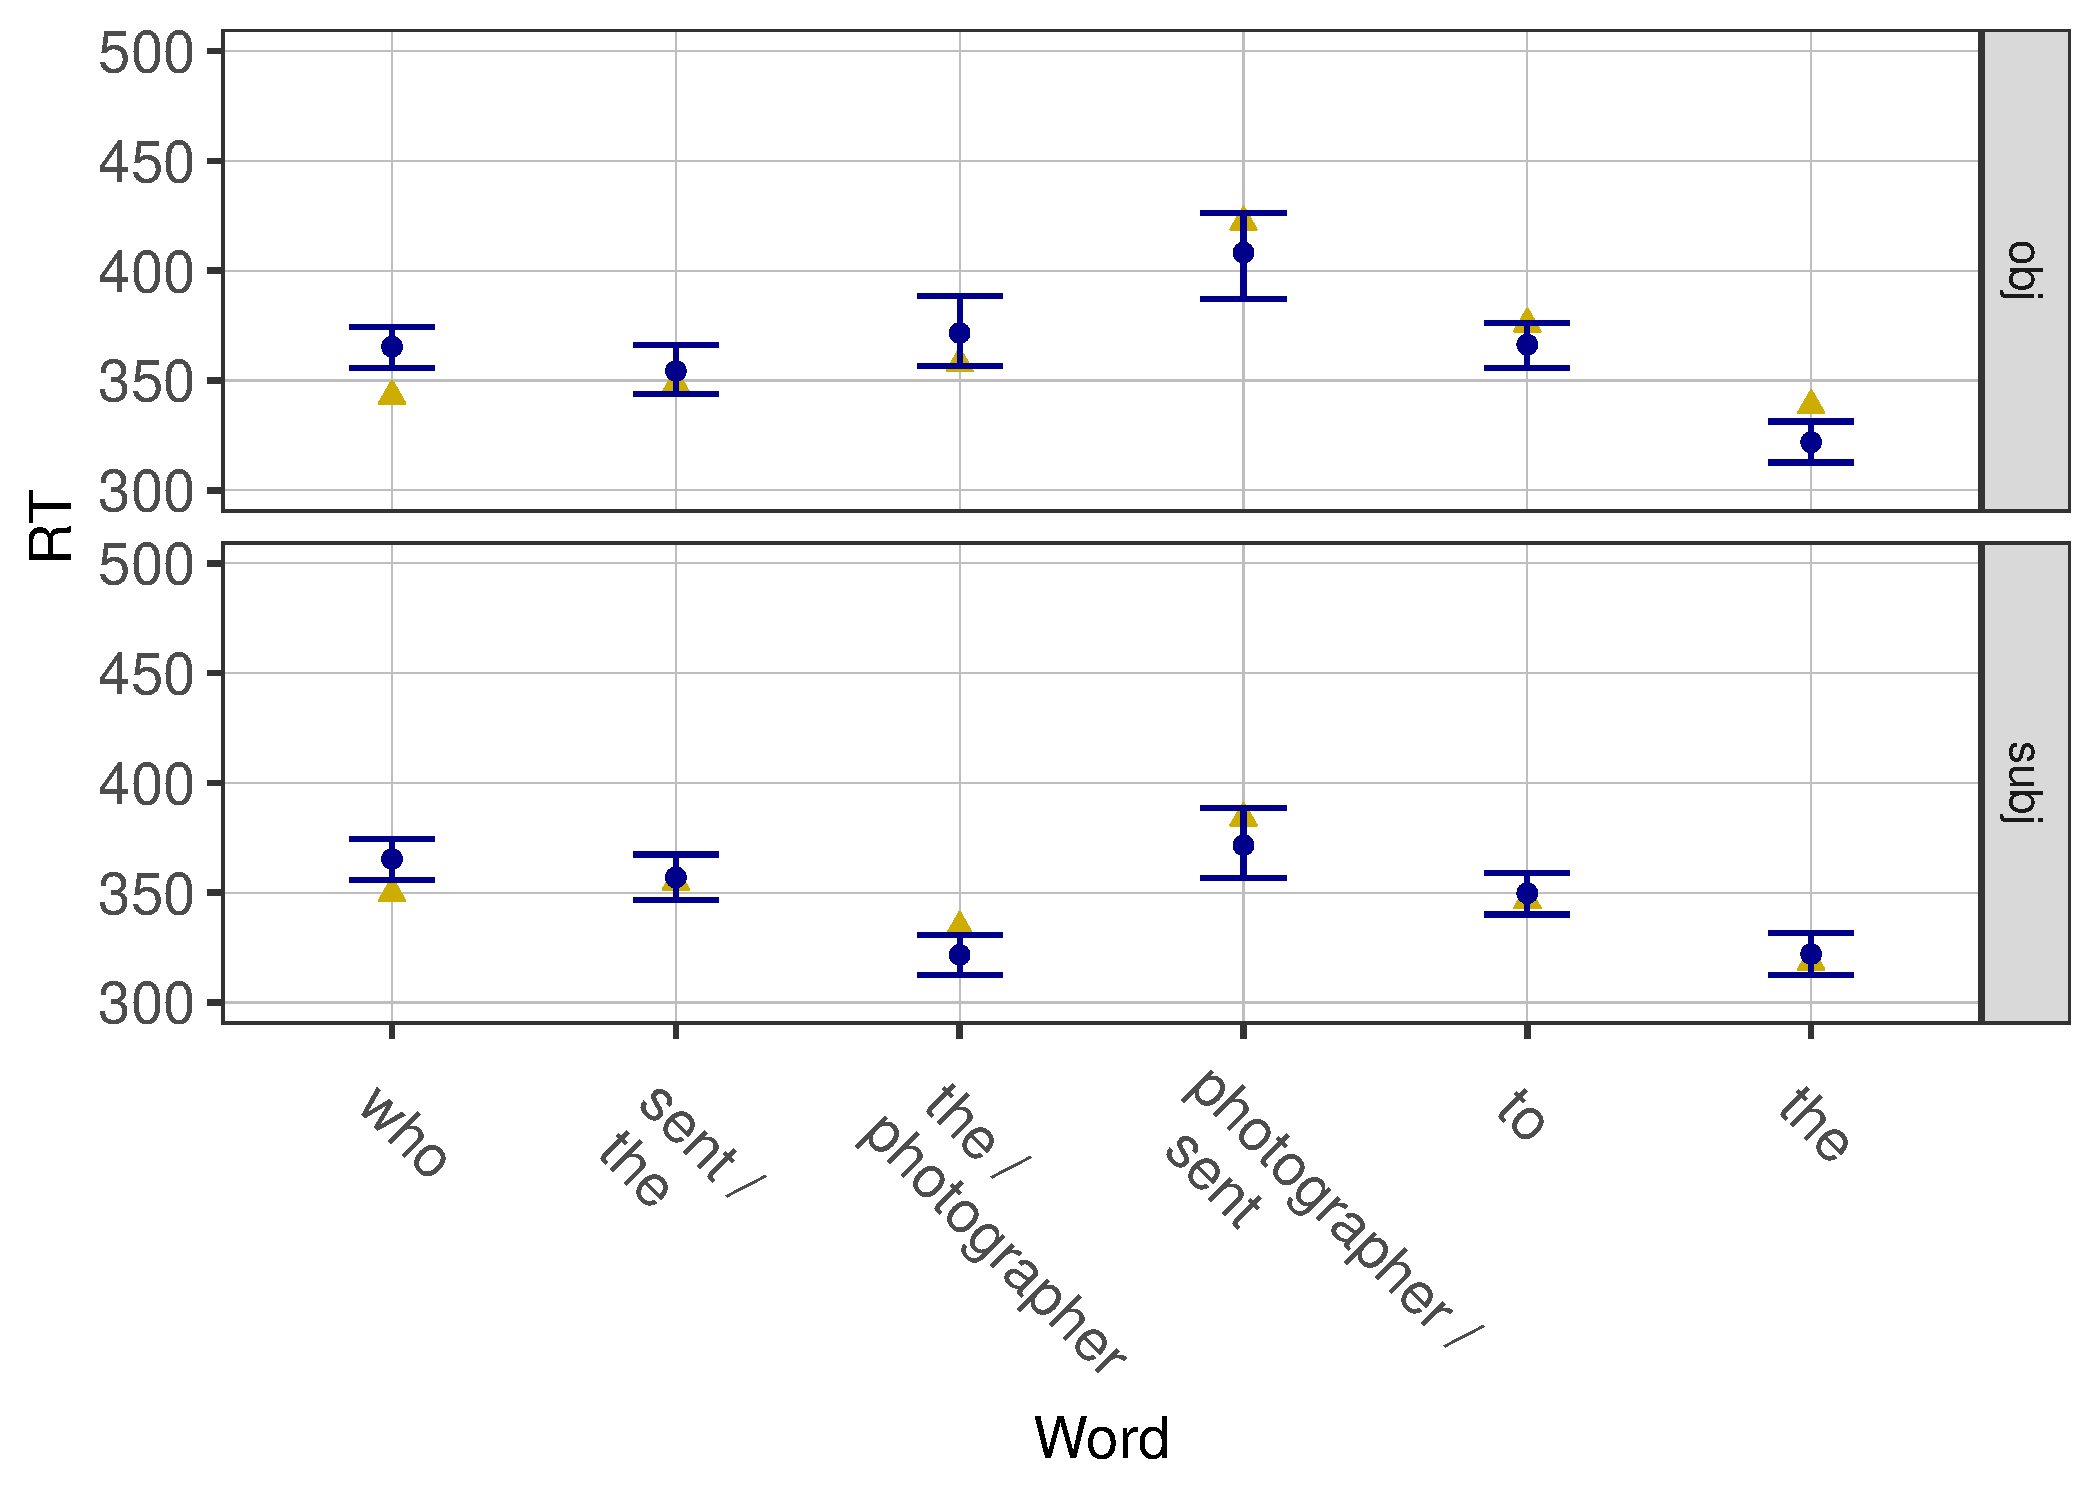
\includegraphics[width=\maxwidth]{figures/figure7regionsunnamed-chunk-5-1} 

\end{knitrout}


\begin{knitrout}
\definecolor{shadecolor}{rgb}{0.969, 0.969, 0.969}\color{fgcolor}\begin{kframe}
\begin{alltt}
\hlkwd{ggsave}\hlstd{(}\hlstr{"predictions-observed-RT-grodner-gibson-exp1-6regions.pdf"}\hlstd{,} \hlkwc{width} \hlstd{=} \hlnum{20}\hlstd{,}
    \hlkwc{height} \hlstd{=} \hlnum{12}\hlstd{)}
\end{alltt}
\end{kframe}
\end{knitrout}

\section{WAIC}

\begin{knitrout}
\definecolor{shadecolor}{rgb}{0.969, 0.969, 0.969}\color{fgcolor}\begin{kframe}
\begin{alltt}
\hlstd{calculate_log_likelihood} \hlkwb{<-} \hlkwa{function}\hlstd{(}\hlkwc{predicted}\hlstd{,} \hlkwc{observed}\hlstd{,} \hlkwc{std}\hlstd{) \{}

    \hlkwd{log}\hlstd{(}\hlkwd{dnorm}\hlstd{(observed,} \hlkwc{mean} \hlstd{= predicted,} \hlkwc{sd} \hlstd{= std))}

\hlstd{\}}

\hlstd{ll} \hlkwb{<-} \hlkwd{matrix}\hlstd{(}\hlkwd{calculate_log_likelihood}\hlstd{(data.all}\hlopt{$}\hlstd{RT, data.all}\hlopt{$}\hlstd{x, data.all}\hlopt{$}\hlstd{std),}
    \hlkwc{nrow} \hlstd{= ndraws)}

\hlkwd{str}\hlstd{(ll)}
\end{alltt}
\begin{verbatim}
##  num [1:10018, 1:12] -4.47 -4.47 -4.47 -4.3 -4.21 ...
\end{verbatim}
\begin{alltt}
\hlkwd{waic}\hlstd{(ll)}
\end{alltt}


{\ttfamily\noindent\color{warningcolor}{\#\# Warning: \\\#\# 2 (16.7\%) p\_waic estimates greater than 0.4. We recommend trying loo instead.}}\begin{verbatim}
## 
## Computed from 10018 by 12 log-likelihood matrix
## 
##           Estimate  SE
## elpd_waic    -51.0 1.5
## p_waic         2.6 0.6
## waic         102.0 3.0
## 
## 2 (16.7%) p_waic estimates greater than 0.4. We recommend trying loo instead.
\end{verbatim}
\end{kframe}
\end{knitrout}
\section{Posterior predictive checks}

\begin{knitrout}
\definecolor{shadecolor}{rgb}{0.969, 0.969, 0.969}\color{fgcolor}\begin{kframe}
\begin{alltt}
\hlstd{dataf} \hlkwb{<-} \hlkwd{read.csv}\hlstd{(}\hlstr{"chain1/posterior_predictive_checks_subj.csv"}\hlstd{,} \hlkwc{row.names} \hlstd{=} \hlnum{1}\hlstd{)}

\hlkwd{str}\hlstd{(dataf)}
\end{alltt}
\begin{verbatim}
## 'data.frame':	5507 obs. of  6 variables:
##  $ X0: num  422 383 349 386 374 ...
##  $ X1: num  354 358 388 380 317 ...
##  $ X2: num  363 315 362 317 298 ...
##  $ X3: num  373 338 412 388 319 ...
##  $ X4: num  400 403 381 400 392 ...
##  $ X5: num  346 365 360 295 346 ...
\end{verbatim}
\begin{alltt}
\hlstd{dataf2} \hlkwb{<-} \hlkwd{read.csv}\hlstd{(}\hlstr{"chain1/posterior_predictive_checks_obj.csv"}\hlstd{,} \hlkwc{row.names} \hlstd{=} \hlnum{1}\hlstd{)}

\hlkwd{str}\hlstd{(dataf2)}
\end{alltt}
\begin{verbatim}
## 'data.frame':	5507 obs. of  6 variables:
##  $ X0: num  340 357 363 363 386 ...
##  $ X1: num  382 409 389 369 372 ...
##  $ X2: num  407 361 485 363 385 ...
##  $ X3: num  372 358 356 424 402 ...
##  $ X4: num  405 402 360 319 342 ...
##  $ X5: num  308 344 404 328 392 ...
\end{verbatim}
\begin{alltt}
\hlstd{dataf.c2} \hlkwb{<-} \hlkwd{read.csv}\hlstd{(}\hlstr{"chain2/posterior_predictive_checks_subj.csv"}\hlstd{,} \hlkwc{row.names} \hlstd{=} \hlnum{1}\hlstd{)}

\hlstd{dataf} \hlkwb{<-} \hlkwd{rbind}\hlstd{(dataf, dataf.c2)}

\hlkwd{str}\hlstd{(dataf)}
\end{alltt}
\begin{verbatim}
## 'data.frame':	11014 obs. of  6 variables:
##  $ X0: num  422 383 349 386 374 ...
##  $ X1: num  354 358 388 380 317 ...
##  $ X2: num  363 315 362 317 298 ...
##  $ X3: num  373 338 412 388 319 ...
##  $ X4: num  400 403 381 400 392 ...
##  $ X5: num  346 365 360 295 346 ...
\end{verbatim}
\begin{alltt}
\hlstd{dataf2.c2} \hlkwb{<-} \hlkwd{read.csv}\hlstd{(}\hlstr{"chain2/posterior_predictive_checks_obj.csv"}\hlstd{,} \hlkwc{row.names} \hlstd{=} \hlnum{1}\hlstd{)}

\hlstd{dataf2} \hlkwb{<-} \hlkwd{rbind}\hlstd{(dataf2, dataf2.c2)}

\hlkwd{str}\hlstd{(dataf)}
\end{alltt}
\begin{verbatim}
## 'data.frame':	11014 obs. of  6 variables:
##  $ X0: num  422 383 349 386 374 ...
##  $ X1: num  354 358 388 380 317 ...
##  $ X2: num  363 315 362 317 298 ...
##  $ X3: num  373 338 412 388 319 ...
##  $ X4: num  400 403 381 400 392 ...
##  $ X5: num  346 365 360 295 346 ...
\end{verbatim}
\begin{alltt}
\hlstd{ndraws} \hlkwb{<-} \hlkwd{length}\hlstd{(dataf2[,} \hlnum{1}\hlstd{])}

\hlstd{data.all} \hlkwb{<-} \hlkwd{data.frame}\hlstd{(}\hlkwc{word_no} \hlstd{=} \hlkwd{rep.int}\hlstd{(}\hlkwd{rep}\hlstd{(}\hlkwd{paste}\hlstd{(}\hlstr{"No"}\hlstd{,} \hlnum{3}\hlopt{:}\hlnum{8}\hlstd{,} \hlkwc{sep} \hlstd{=} \hlstr{""}\hlstd{),} \hlkwc{each} \hlstd{= ndraws),}
    \hlnum{2}\hlstd{),} \hlkwc{word} \hlstd{=} \hlkwd{factor}\hlstd{(}\hlkwd{rep}\hlstd{(}\hlkwd{rep}\hlstd{(}\hlkwd{c}\hlstd{(}\hlstr{"who"}\hlstd{,} \hlstr{"sent /\textbackslash{}nthe"}\hlstd{,} \hlstr{"the /\textbackslash{}nphotographer"}\hlstd{,}
    \hlstr{"photographer /\textbackslash{}nsent"}\hlstd{,} \hlstr{"to"}\hlstd{,} \hlstr{"the"}\hlstd{),} \hlkwc{each} \hlstd{= ndraws),} \hlnum{2}\hlstd{),} \hlkwc{levels} \hlstd{=} \hlkwd{c}\hlstd{(}\hlstr{"who"}\hlstd{,}
    \hlstr{"sent /\textbackslash{}nthe"}\hlstd{,} \hlstr{"the /\textbackslash{}nphotographer"}\hlstd{,} \hlstr{"photographer /\textbackslash{}nsent"}\hlstd{,} \hlstr{"to"}\hlstd{,} \hlstr{"the"}\hlstd{)),}
    \hlkwc{extraction} \hlstd{=} \hlkwd{c}\hlstd{(}\hlkwd{rep}\hlstd{(}\hlstr{"subj"}\hlstd{, ndraws} \hlopt{*} \hlnum{6}\hlstd{),} \hlkwd{rep}\hlstd{(}\hlstr{"obj"}\hlstd{, ndraws} \hlopt{*} \hlnum{6}\hlstd{)),} \hlkwc{RT} \hlstd{=} \hlkwd{c}\hlstd{(dataf[,}
        \hlnum{1}\hlstd{], dataf[,} \hlnum{2}\hlstd{], dataf[,} \hlnum{3}\hlstd{], dataf[,} \hlnum{4}\hlstd{], dataf[,} \hlnum{5}\hlstd{], dataf[,} \hlnum{6}\hlstd{], dataf2[,}
        \hlnum{1}\hlstd{], dataf2[,} \hlnum{2}\hlstd{], dataf2[,} \hlnum{3}\hlstd{], dataf2[,} \hlnum{4}\hlstd{], dataf2[,} \hlnum{5}\hlstd{], dataf2[,} \hlnum{6}\hlstd{]),}
    \hlkwc{x} \hlstd{=} \hlkwd{rep}\hlstd{(}\hlkwd{c}\hlstd{(}\hlnum{349.8}\hlstd{,} \hlnum{354.8}\hlstd{,} \hlnum{334.3}\hlstd{,} \hlnum{384}\hlstd{,} \hlnum{346.5}\hlstd{,} \hlnum{318.4}\hlstd{,} \hlnum{343}\hlstd{,} \hlnum{348.1}\hlstd{,} \hlnum{357.6}\hlstd{,} \hlnum{422.1}\hlstd{,}
        \hlnum{375.8}\hlstd{,} \hlnum{338.6}\hlstd{),} \hlkwc{each} \hlstd{= ndraws))}

\hlkwd{str}\hlstd{(data.all)}
\end{alltt}
\begin{verbatim}
## 'data.frame':	132168 obs. of  5 variables:
##  $ word_no   : Factor w/ 6 levels "No3","No4","No5",..: 1 1 1 1 1 1 1 1 1 1 ...
##  $ word      : Factor w/ 6 levels "who","sent /\nthe",..: 1 1 1 1 1 1 1 1 1 1 ...
##  $ extraction: Factor w/ 2 levels "obj","subj": 2 2 2 2 2 2 2 2 2 2 ...
##  $ RT        : num  422 383 349 386 374 ...
##  $ x         : num  350 350 350 350 350 ...
\end{verbatim}
\begin{alltt}
\hlcom{# data.all <- subset(data.all, RT > 50 & RT < 3000)}

\hlkwd{library}\hlstd{(ggplot2)}

\hlkwd{library}\hlstd{(dplyr)}

\hlstd{data.to.plot} \hlkwb{<-} \hlstd{data.all} \hlopt \hlkwd{group_by}\hlstd{(extraction, word_no)} \hlopt \hlkwd{summarise}\hlstd{(}\hlkwc{Extraction} \hlstd{=} \hlkwd{first}\hlstd{(extraction),}
    \hlkwc{Word.no} \hlstd{=} \hlkwd{as.factor}\hlstd{(}\hlkwd{first}\hlstd{(word_no)),} \hlkwc{Word} \hlstd{=} \hlkwd{as.factor}\hlstd{(}\hlkwd{first}\hlstd{(word)),} \hlkwc{CF1} \hlstd{=} \hlkwd{quantile}\hlstd{(RT,}
        \hlkwc{probs} \hlstd{=} \hlkwd{c}\hlstd{(}\hlnum{0.05}\hlstd{,} \hlnum{0.95}\hlstd{))[}\hlnum{1}\hlstd{],} \hlkwc{CF2} \hlstd{=} \hlkwd{quantile}\hlstd{(RT,} \hlkwc{probs} \hlstd{=} \hlkwd{c}\hlstd{(}\hlnum{0.05}\hlstd{,} \hlnum{0.95}\hlstd{))[}\hlnum{2}\hlstd{],}
    \hlkwc{RT} \hlstd{=} \hlkwd{mean}\hlstd{(RT),} \hlkwc{Observed} \hlstd{=} \hlkwd{first}\hlstd{(x))}
\end{alltt}


{\ttfamily\noindent\itshape\color{messagecolor}{\#\# `summarise()` has grouped output by 'extraction'. You can override using the `.groups` argument.}}\begin{alltt}
\hlstd{data.to.plot}
\end{alltt}
\begin{verbatim}
## # A tibble: 12 x 9
## # Groups:   extraction [2]
##    extraction word_no Extraction Word.no Word     CF1   CF2    RT Observed
##    <fct>      <fct>   <fct>      <fct>   <fct>  <dbl> <dbl> <dbl>    <dbl>
##  1 obj        No3     obj        No3     "who"   336.  393.  365.     343 
##  2 obj        No4     obj        No4     "sent~  326.  384.  354.     348.
##  3 obj        No5     obj        No5     "the ~  341.  404.  372.     358.
##  4 obj        No6     obj        No6     "phot~  374.  440.  408.     422.
##  5 obj        No7     obj        No7     "to"    337.  395.  366.     376.
##  6 obj        No8     obj        No8     "the"   293.  351.  322.     339.
##  7 subj       No3     subj       No3     "who"   337.  393.  365.     350.
##  8 subj       No4     subj       No4     "sent~  328.  386.  357.     355.
##  9 subj       No5     subj       No5     "the ~  293.  350.  322.     334.
## 10 subj       No6     subj       No6     "phot~  340.  404.  372.     384 
## 11 subj       No7     subj       No7     "to"    322.  379.  350.     346.
## 12 subj       No8     subj       No8     "the"   293.  350.  322.     318.
\end{verbatim}
\begin{alltt}
\hlstd{g1} \hlkwb{<-} \hlkwd{ggplot}\hlstd{(data.to.plot,} \hlkwd{aes}\hlstd{(Word, RT))}
\hlstd{g1} \hlkwb{<-} \hlstd{g1} \hlopt{+} \hlkwd{geom_point}\hlstd{(}\hlkwd{aes}\hlstd{(}\hlkwc{x} \hlstd{= Word,} \hlkwc{y} \hlstd{= Observed),} \hlkwc{fill} \hlstd{=} \hlstr{"gold3"}\hlstd{,} \hlkwc{color} \hlstd{=} \hlstr{"gold3"}\hlstd{,}
    \hlkwc{pch} \hlstd{=} \hlnum{24}\hlstd{,} \hlkwc{size} \hlstd{=} \hlnum{4}\hlstd{)} \hlopt{+} \hlkwd{geom_point}\hlstd{(}\hlkwc{color} \hlstd{=} \hlstr{"blue4"}\hlstd{,} \hlkwc{size} \hlstd{=} \hlkwd{I}\hlstd{(}\hlnum{4}\hlstd{))} \hlopt{+} \hlkwd{geom_errorbar}\hlstd{(}\hlkwd{aes}\hlstd{(}\hlkwc{ymin} \hlstd{= CF1,}
    \hlkwc{ymax} \hlstd{= CF2),} \hlkwc{color} \hlstd{=} \hlstr{"blue4"}\hlstd{,} \hlkwc{width} \hlstd{=} \hlnum{0.3}\hlstd{,} \hlkwc{size} \hlstd{=} \hlkwd{I}\hlstd{(}\hlnum{1.2}\hlstd{))} \hlopt{+} \hlkwd{theme_bw}\hlstd{(}\hlnum{28}\hlstd{)}
\hlstd{g1} \hlkwb{<-} \hlstd{g1} \hlopt{+} \hlkwd{theme}\hlstd{(}\hlkwc{axis.text.x} \hlstd{=} \hlkwd{element_text}\hlstd{(}\hlkwc{angle} \hlstd{=} \hlopt{-}\hlnum{45}\hlstd{,} \hlkwc{hjust} \hlstd{=} \hlnum{0.1}\hlstd{,} \hlkwc{size} \hlstd{=} \hlnum{28}\hlstd{),}
    \hlkwc{axis.text.y} \hlstd{=} \hlkwd{element_text}\hlstd{(}\hlkwc{size} \hlstd{=} \hlnum{28}\hlstd{),} \hlkwc{axis.title} \hlstd{=} \hlkwd{element_text}\hlstd{(}\hlkwc{size} \hlstd{=} \hlnum{28}\hlstd{),}
    \hlkwc{legend.position} \hlstd{=} \hlstr{"none"}\hlstd{,} \hlkwc{panel.grid.major} \hlstd{=} \hlkwd{element_line}\hlstd{(}\hlkwc{colour} \hlstd{=} \hlstr{"grey"}\hlstd{,}
        \hlkwc{size} \hlstd{= (}\hlnum{0.25}\hlstd{)),} \hlkwc{panel.grid.minor} \hlstd{=} \hlkwd{element_blank}\hlstd{())}
\hlstd{g1} \hlkwb{<-} \hlstd{g1} \hlopt{+} \hlkwd{coord_cartesian}\hlstd{(}\hlkwc{ylim} \hlstd{=} \hlkwd{c}\hlstd{(}\hlnum{250}\hlstd{,} \hlnum{500}\hlstd{))} \hlopt{+} \hlkwd{facet_grid}\hlstd{(Extraction} \hlopt{~} \hlstd{.)}
\end{alltt}
\end{kframe}
\end{knitrout}

\begin{knitrout}
\definecolor{shadecolor}{rgb}{0.969, 0.969, 0.969}\color{fgcolor}
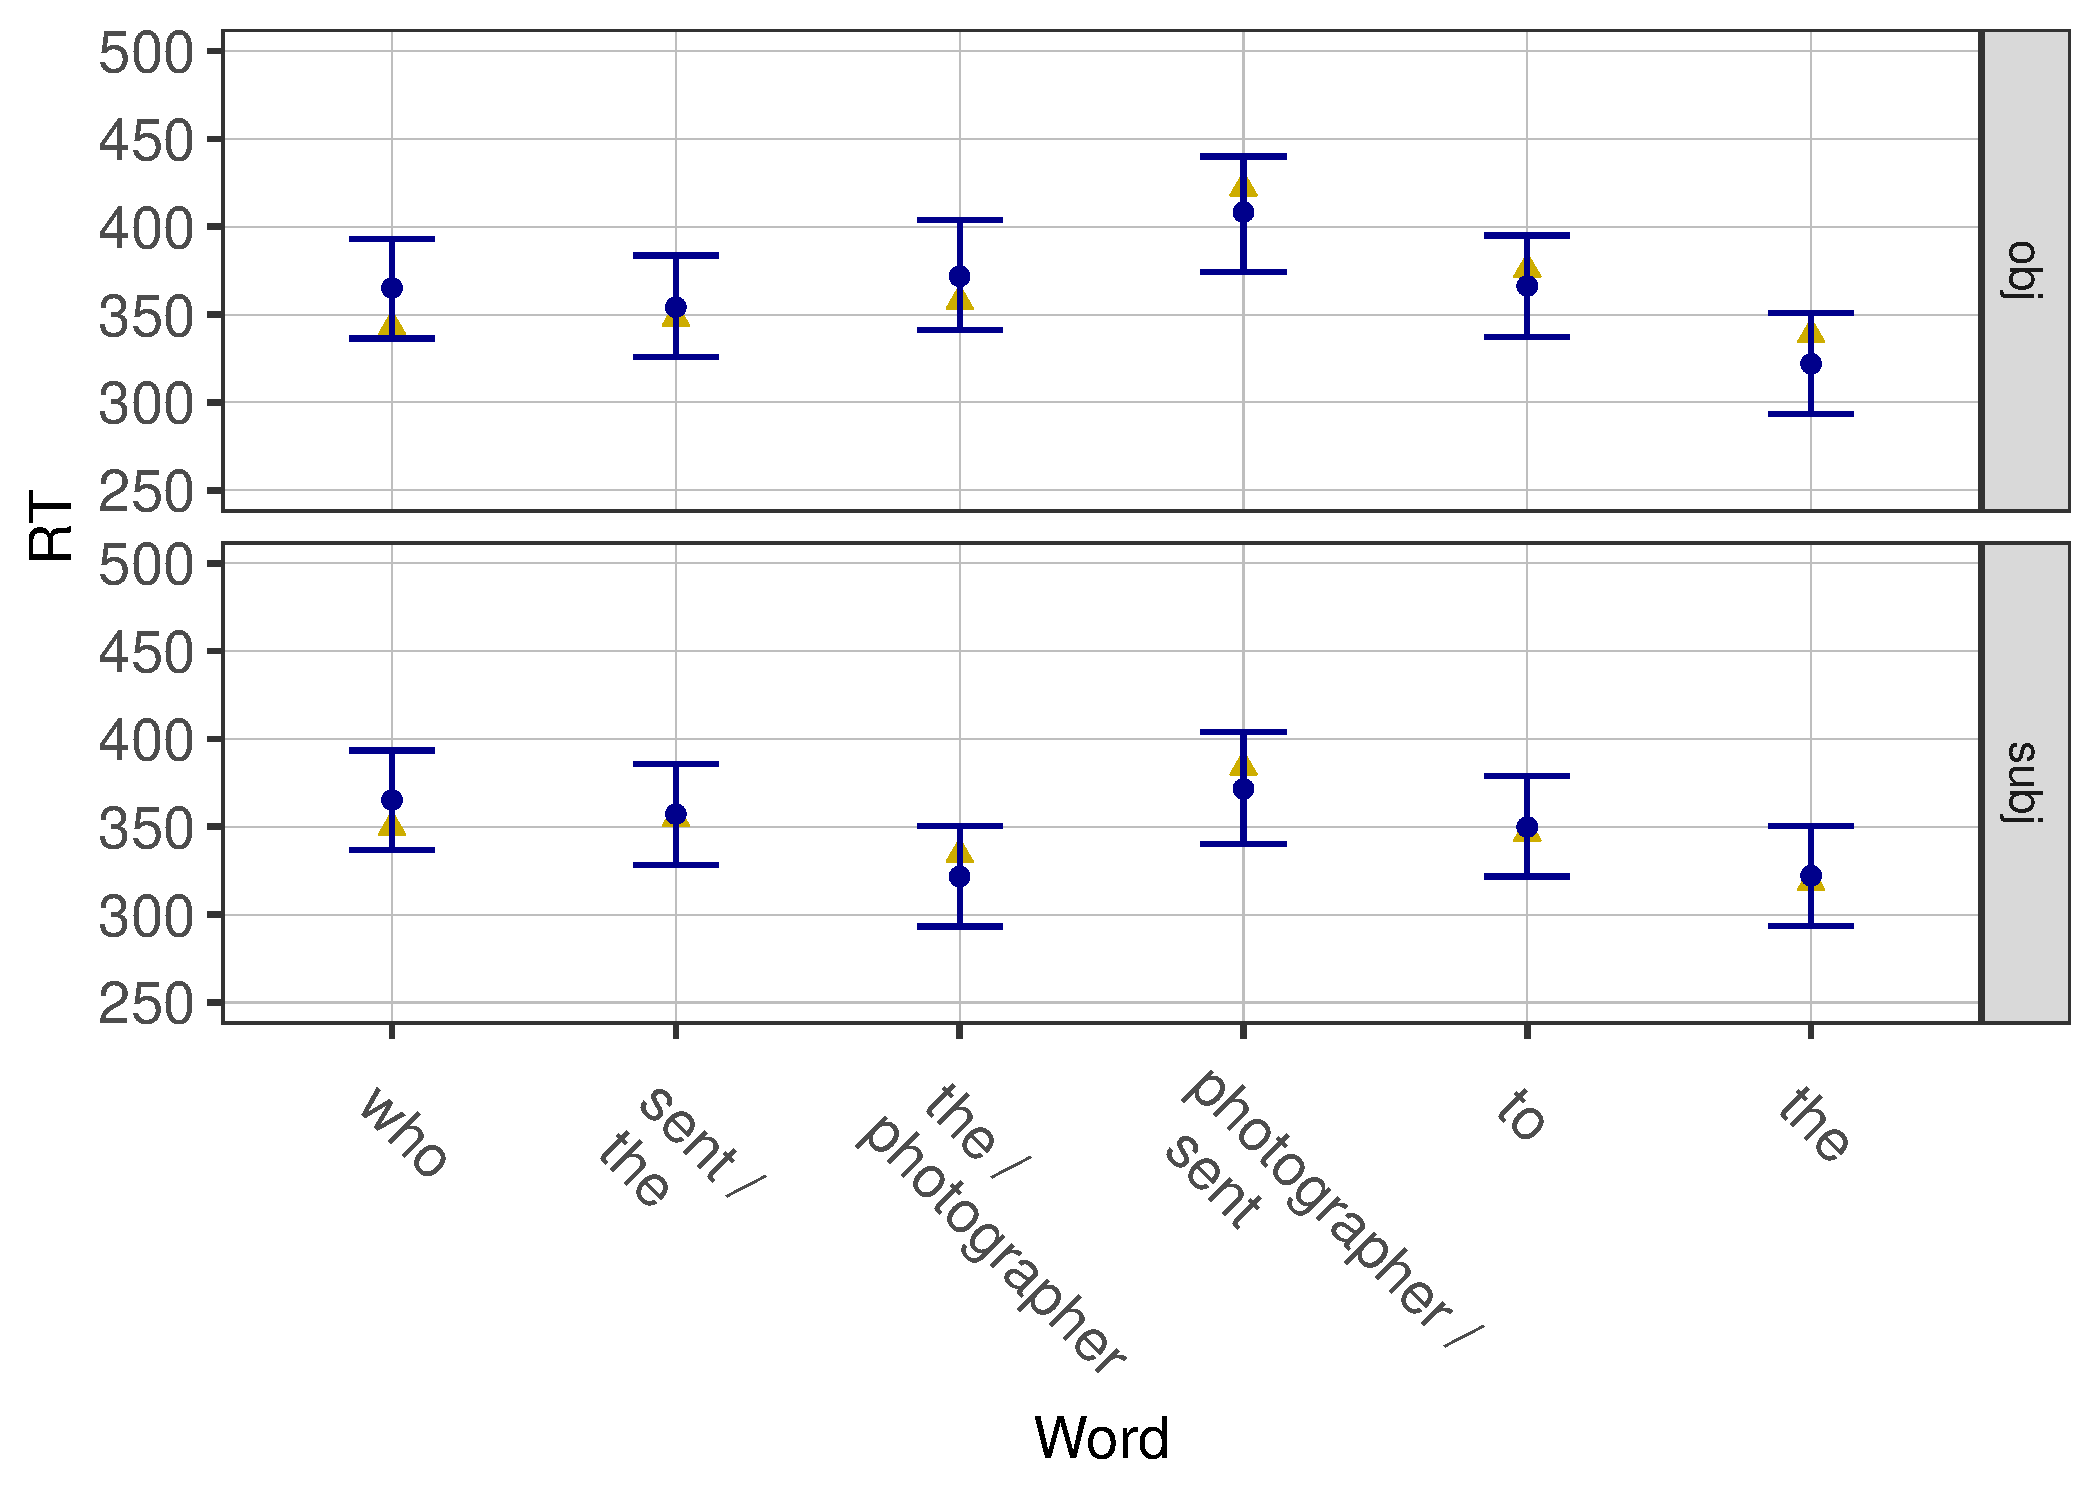
\includegraphics[width=\maxwidth]{figures/figure7regionsunnamed-chunk-9-1} 

\end{knitrout}


\begin{knitrout}
\definecolor{shadecolor}{rgb}{0.969, 0.969, 0.969}\color{fgcolor}\begin{kframe}
\begin{alltt}
\hlkwd{ggsave}\hlstd{(}\hlstr{"posterior-predictive-checks-grodner-gibson-exp1-6regions.pdf"}\hlstd{,} \hlkwc{width} \hlstd{=} \hlnum{20}\hlstd{,}
    \hlkwc{height} \hlstd{=} \hlnum{12}\hlstd{)}
\end{alltt}
\end{kframe}
\end{knitrout}


\section{Parameters}



\subsection{LF}

Rhat:
\begin{knitrout}
\definecolor{shadecolor}{rgb}{0.969, 0.969, 0.969}\color{fgcolor}\begin{kframe}
\begin{alltt}
\hlstd{draws} \hlkwb{<-} \hlkwd{createdraws}\hlstd{(}\hlstr{"lf"}\hlstd{)}
\end{alltt}


{\ttfamily\noindent\itshape\color{messagecolor}{\#\# Note: Using an external vector in selections is ambiguous.\\\#\# i Use `all\_of(param)` instead of `param` to silence this message.\\\#\# i See <https://tidyselect.r-lib.org/reference/faq-external-vector.html>.\\\#\# This message is displayed once per session.}}\begin{alltt}
\hlkwd{str}\hlstd{(draws)}
\end{alltt}
\begin{verbatim}
##  num [1:5009, 1:2] 0.0239 0.0239 0.022 0.022 0.0234 ...
\end{verbatim}
\begin{alltt}
\hlkwd{Rhat}\hlstd{(draws)}
\end{alltt}
\begin{verbatim}
## [1] 1.047399
\end{verbatim}
\end{kframe}
\end{knitrout}

Mean etc.

\begin{knitrout}
\definecolor{shadecolor}{rgb}{0.969, 0.969, 0.969}\color{fgcolor}\begin{kframe}
\begin{alltt}
\hlkwd{tail}\hlstd{(draws)}
\end{alltt}
\begin{verbatim}
##               [,1]       [,2]
## [5004,] 0.06038476 0.04922450
## [5005,] 0.06038476 0.04922450
## [5006,] 0.06038476 0.04922450
## [5007,] 0.06038476 0.03871595
## [5008,] 0.06038476 0.03871595
## [5009,] 0.06038476 0.03871595
\end{verbatim}
\begin{alltt}
\hlkwd{mean}\hlstd{(}\hlkwd{c}\hlstd{(draws[,} \hlnum{1}\hlopt{:}\hlnum{2}\hlstd{]))}
\end{alltt}
\begin{verbatim}
## [1] 0.04691501
\end{verbatim}
\begin{alltt}
\hlkwd{median}\hlstd{(}\hlkwd{c}\hlstd{(draws[,} \hlnum{1}\hlopt{:}\hlnum{2}\hlstd{]))}
\end{alltt}
\begin{verbatim}
## [1] 0.04912666
\end{verbatim}
\begin{alltt}
\hlkwd{sd}\hlstd{(}\hlkwd{c}\hlstd{(draws[,} \hlnum{1}\hlopt{:}\hlnum{2}\hlstd{]))}
\end{alltt}
\begin{verbatim}
## [1] 0.0121508
\end{verbatim}
\begin{alltt}
\hlstd{g1} \hlkwb{<-} \hlkwd{ggplot}\hlstd{(}\hlkwd{data.frame}\hlstd{(}\hlkwc{latency_factor} \hlstd{=} \hlkwd{c}\hlstd{(draws[,} \hlnum{1}\hlopt{:}\hlnum{2}\hlstd{])),} \hlkwd{aes}\hlstd{(latency_factor))}
\hlstd{g1} \hlkwb{<-} \hlstd{g1} \hlopt{+} \hlkwd{geom_histogram}\hlstd{()} \hlopt{+} \hlkwd{theme_bw}\hlstd{(}\hlnum{28}\hlstd{)}
\hlstd{g1}
\end{alltt}


{\ttfamily\noindent\itshape\color{messagecolor}{\#\# `stat\_bin()` using `bins = 30`. Pick better value with `binwidth`.}}\end{kframe}
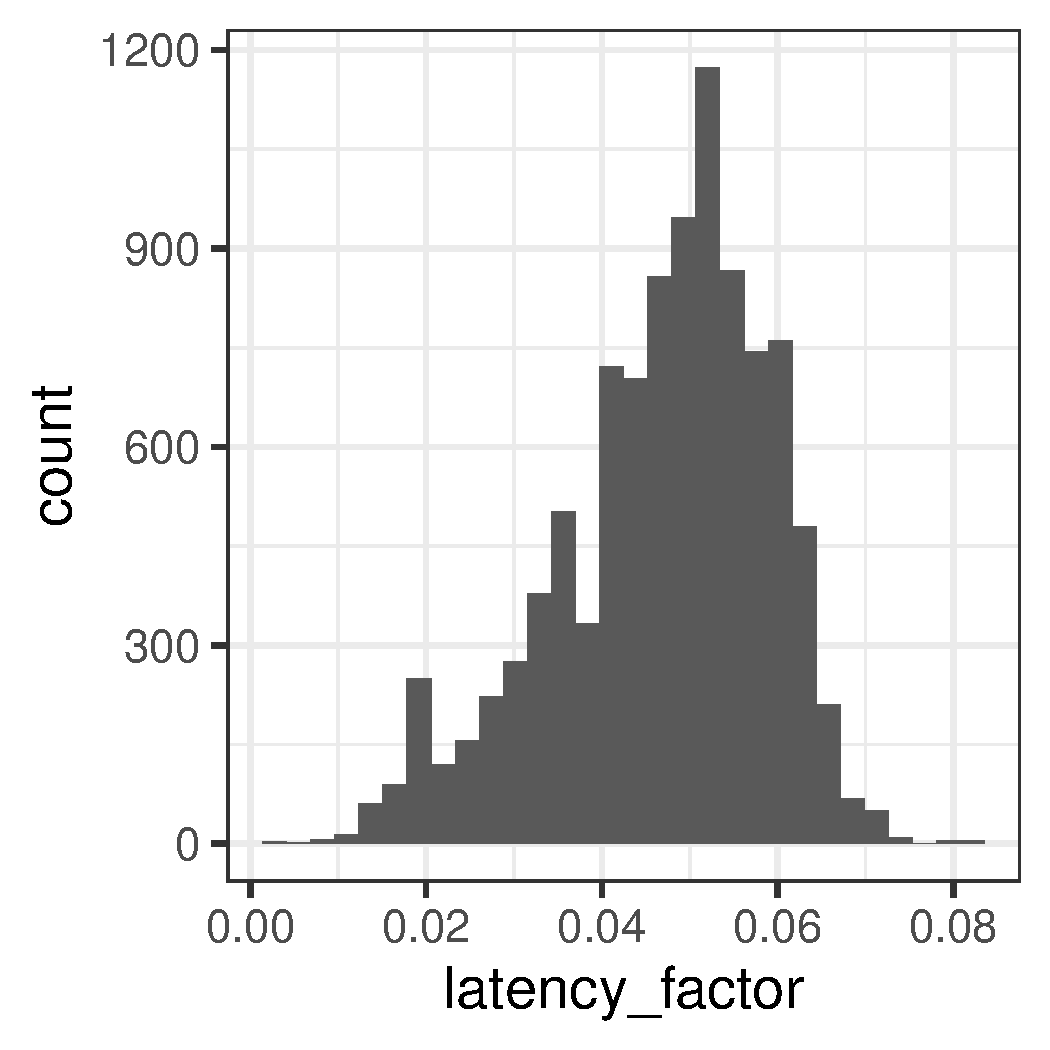
\includegraphics[width=\maxwidth]{figures/figure7regionsunnamed-chunk-13-1} 
\begin{kframe}\begin{alltt}
\hlkwd{ggsave}\hlstd{(}\hlstr{"gg1-lf.pdf"}\hlstd{,} \hlkwc{width} \hlstd{=} \hlnum{20}\hlstd{,} \hlkwc{height} \hlstd{=} \hlnum{12}\hlstd{)}
\end{alltt}


{\ttfamily\noindent\itshape\color{messagecolor}{\#\# `stat\_bin()` using `bins = 30`. Pick better value with `binwidth`.}}\end{kframe}
\end{knitrout}

\subsection{LE}

Rhat:
\begin{knitrout}
\definecolor{shadecolor}{rgb}{0.969, 0.969, 0.969}\color{fgcolor}\begin{kframe}
\begin{alltt}
\hlstd{draws} \hlkwb{<-} \hlkwd{createdraws}\hlstd{(}\hlstr{"le"}\hlstd{)}

\hlkwd{Rhat}\hlstd{(draws)}
\end{alltt}
\begin{verbatim}
## [1] 1.017002
\end{verbatim}
\end{kframe}
\end{knitrout}

Mean etc.

\begin{knitrout}
\definecolor{shadecolor}{rgb}{0.969, 0.969, 0.969}\color{fgcolor}\begin{kframe}
\begin{alltt}
\hlkwd{tail}\hlstd{(draws)}
\end{alltt}
\begin{verbatim}
##              [,1]      [,2]
## [5004,] 0.1273843 0.1619161
## [5005,] 0.1685181 0.1619161
## [5006,] 0.1685181 0.1619161
## [5007,] 0.1685181 0.1619161
## [5008,] 0.1685181 0.1619161
## [5009,] 0.1816423 0.1097034
\end{verbatim}
\begin{alltt}
\hlkwd{mean}\hlstd{(}\hlkwd{c}\hlstd{(draws[,} \hlnum{1}\hlopt{:}\hlnum{2}\hlstd{]))}
\end{alltt}
\begin{verbatim}
## [1] 0.1703266
\end{verbatim}
\begin{alltt}
\hlkwd{median}\hlstd{(}\hlkwd{c}\hlstd{(draws[,} \hlnum{1}\hlopt{:}\hlnum{2}\hlstd{]))}
\end{alltt}
\begin{verbatim}
## [1] 0.1511095
\end{verbatim}
\begin{alltt}
\hlkwd{sd}\hlstd{(}\hlkwd{c}\hlstd{(draws[,} \hlnum{1}\hlopt{:}\hlnum{2}\hlstd{]))}
\end{alltt}
\begin{verbatim}
## [1] 0.07967335
\end{verbatim}
\begin{alltt}
\hlstd{g1} \hlkwb{<-} \hlkwd{ggplot}\hlstd{(}\hlkwd{data.frame}\hlstd{(}\hlkwc{latency_exponent} \hlstd{=} \hlkwd{c}\hlstd{(draws[,} \hlnum{1}\hlopt{:}\hlnum{2}\hlstd{])),} \hlkwd{aes}\hlstd{(latency_exponent))}
\hlstd{g1} \hlkwb{<-} \hlstd{g1} \hlopt{+} \hlkwd{geom_histogram}\hlstd{()} \hlopt{+} \hlkwd{theme_bw}\hlstd{(}\hlnum{28}\hlstd{)}
\hlstd{g1}
\end{alltt}


{\ttfamily\noindent\itshape\color{messagecolor}{\#\# `stat\_bin()` using `bins = 30`. Pick better value with `binwidth`.}}\end{kframe}
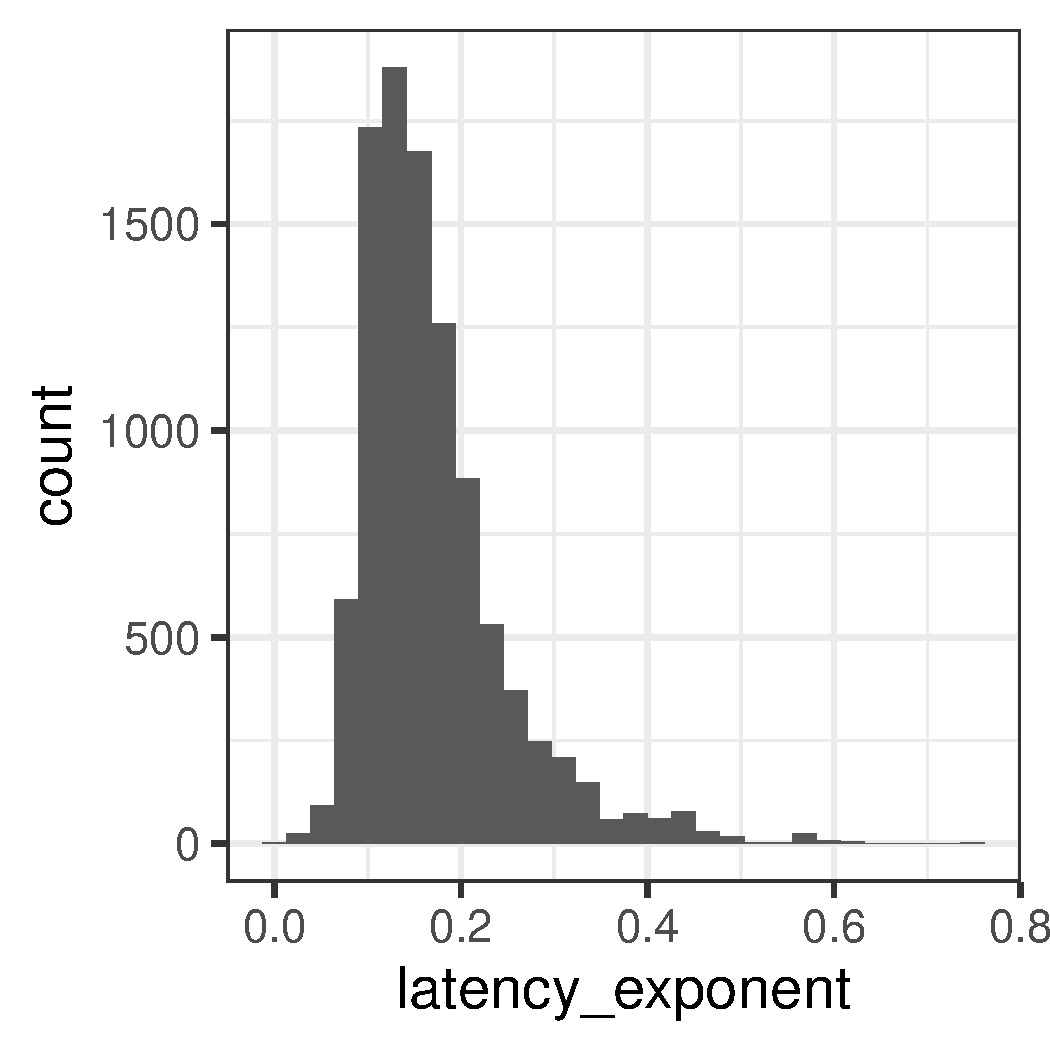
\includegraphics[width=\maxwidth]{figures/figure7regionsunnamed-chunk-15-1} 
\begin{kframe}\begin{alltt}
\hlkwd{ggsave}\hlstd{(}\hlstr{"gg1-le.pdf"}\hlstd{,} \hlkwc{width} \hlstd{=} \hlnum{20}\hlstd{,} \hlkwc{height} \hlstd{=} \hlnum{12}\hlstd{)}
\end{alltt}


{\ttfamily\noindent\itshape\color{messagecolor}{\#\# `stat\_bin()` using `bins = 30`. Pick better value with `binwidth`.}}\end{kframe}
\end{knitrout}

\subsection{RF}

Rhat:
\begin{knitrout}
\definecolor{shadecolor}{rgb}{0.969, 0.969, 0.969}\color{fgcolor}\begin{kframe}
\begin{alltt}
\hlstd{draws} \hlkwb{<-} \hlkwd{createdraws}\hlstd{(}\hlstr{"rf"}\hlstd{)}

\hlkwd{Rhat}\hlstd{(draws)}
\end{alltt}
\begin{verbatim}
## [1] 1.049294
\end{verbatim}
\end{kframe}
\end{knitrout}

Mean etc.

\begin{knitrout}
\definecolor{shadecolor}{rgb}{0.969, 0.969, 0.969}\color{fgcolor}\begin{kframe}
\begin{alltt}
\hlkwd{tail}\hlstd{(draws)}
\end{alltt}
\begin{verbatim}
##               [,1]       [,2]
## [5004,] 0.03094929 0.03350533
## [5005,] 0.03094929 0.03354615
## [5006,] 0.03094929 0.03354615
## [5007,] 0.03094929 0.03354615
## [5008,] 0.03094929 0.03354615
## [5009,] 0.03094929 0.03354615
\end{verbatim}
\begin{alltt}
\hlkwd{mean}\hlstd{(}\hlkwd{c}\hlstd{(draws[,} \hlnum{1}\hlopt{:}\hlnum{2}\hlstd{]))}
\end{alltt}
\begin{verbatim}
## [1] 0.03258386
\end{verbatim}
\begin{alltt}
\hlkwd{median}\hlstd{(}\hlkwd{c}\hlstd{(draws[,} \hlnum{1}\hlopt{:}\hlnum{2}\hlstd{]))}
\end{alltt}
\begin{verbatim}
## [1] 0.03209849
\end{verbatim}
\begin{alltt}
\hlkwd{sd}\hlstd{(}\hlkwd{c}\hlstd{(draws[,} \hlnum{1}\hlopt{:}\hlnum{2}\hlstd{]))}
\end{alltt}
\begin{verbatim}
## [1] 0.002003408
\end{verbatim}
\begin{alltt}
\hlstd{g1} \hlkwb{<-} \hlkwd{ggplot}\hlstd{(}\hlkwd{data.frame}\hlstd{(}\hlkwc{rule_firing} \hlstd{=} \hlkwd{c}\hlstd{(draws[,} \hlnum{1}\hlopt{:}\hlnum{2}\hlstd{])),} \hlkwd{aes}\hlstd{(rule_firing))}
\hlstd{g1} \hlkwb{<-} \hlstd{g1} \hlopt{+} \hlkwd{geom_histogram}\hlstd{()} \hlopt{+} \hlkwd{theme_bw}\hlstd{(}\hlnum{28}\hlstd{)}
\hlstd{g1}
\end{alltt}


{\ttfamily\noindent\itshape\color{messagecolor}{\#\# `stat\_bin()` using `bins = 30`. Pick better value with `binwidth`.}}\end{kframe}
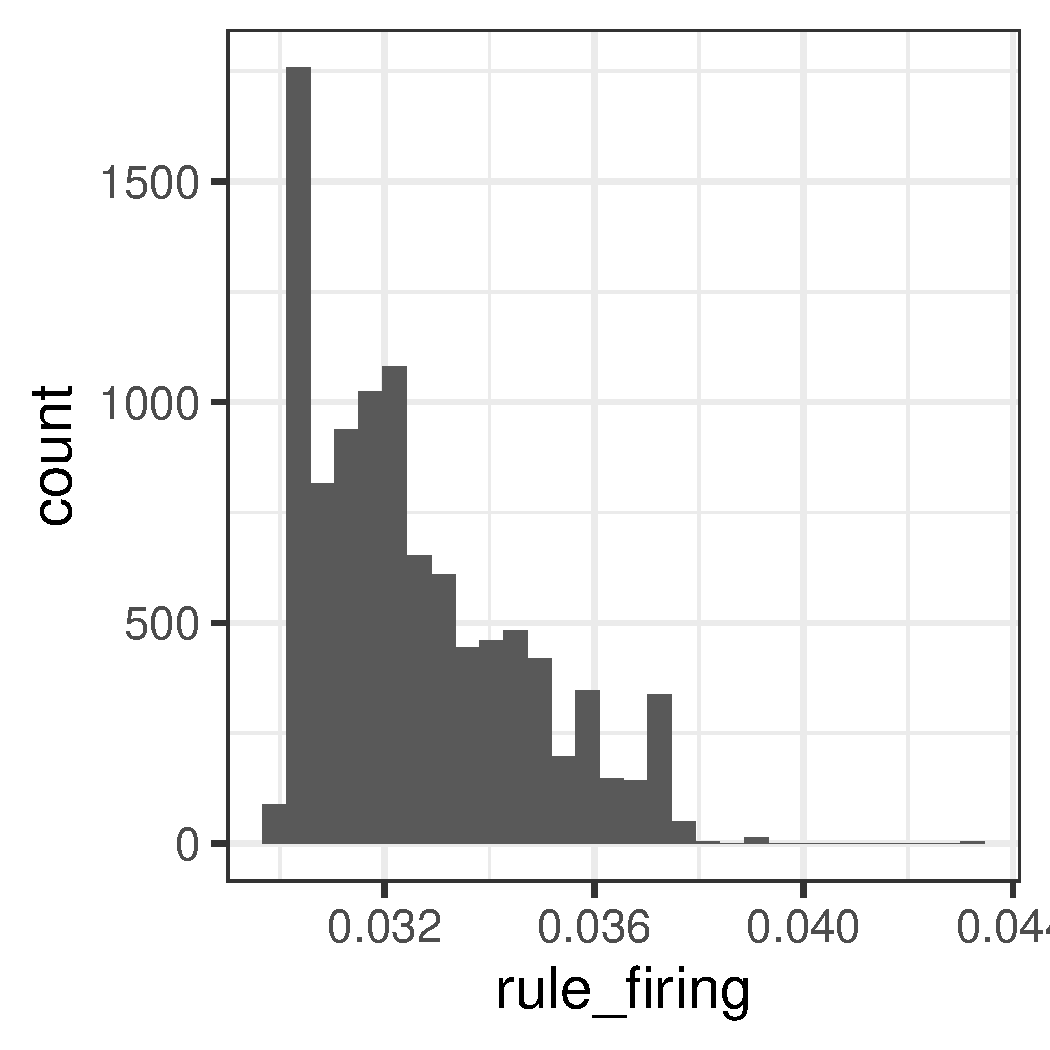
\includegraphics[width=\maxwidth]{figures/figure7regionsunnamed-chunk-17-1} 
\begin{kframe}\begin{alltt}
\hlkwd{ggsave}\hlstd{(}\hlstr{"gg1-rf.pdf"}\hlstd{,} \hlkwc{width} \hlstd{=} \hlnum{20}\hlstd{,} \hlkwc{height} \hlstd{=} \hlnum{12}\hlstd{)}
\end{alltt}


{\ttfamily\noindent\itshape\color{messagecolor}{\#\# `stat\_bin()` using `bins = 30`. Pick better value with `binwidth`.}}\end{kframe}
\end{knitrout}

\subsection{Weight}

Rhat:
\begin{knitrout}
\definecolor{shadecolor}{rgb}{0.969, 0.969, 0.969}\color{fgcolor}\begin{kframe}
\begin{alltt}
\hlstd{draws} \hlkwb{<-} \hlkwd{createdraws}\hlstd{(}\hlstr{"weight"}\hlstd{)}

\hlkwd{Rhat}\hlstd{(draws)}
\end{alltt}
\begin{verbatim}
## [1] 1.010444
\end{verbatim}
\end{kframe}
\end{knitrout}

Mean etc.

\begin{knitrout}
\definecolor{shadecolor}{rgb}{0.969, 0.969, 0.969}\color{fgcolor}\begin{kframe}
\begin{alltt}
\hlkwd{tail}\hlstd{(draws)}
\end{alltt}
\begin{verbatim}
##             [,1]     [,2]
## [5004,] 25.07908 11.08713
## [5005,] 12.75977 11.08713
## [5006,] 12.75977 27.17773
## [5007,] 16.89661 11.15825
## [5008,] 17.30988 21.06276
## [5009,] 29.46745 27.63666
\end{verbatim}
\begin{alltt}
\hlkwd{mean}\hlstd{(}\hlkwd{c}\hlstd{(draws[,} \hlnum{1}\hlopt{:}\hlnum{2}\hlstd{]))}
\end{alltt}
\begin{verbatim}
## [1] 35.37922
\end{verbatim}
\begin{alltt}
\hlkwd{median}\hlstd{(}\hlkwd{c}\hlstd{(draws[,} \hlnum{1}\hlopt{:}\hlnum{2}\hlstd{]))}
\end{alltt}
\begin{verbatim}
## [1] 28.87603
\end{verbatim}
\begin{alltt}
\hlkwd{sd}\hlstd{(}\hlkwd{c}\hlstd{(draws[,} \hlnum{1}\hlopt{:}\hlnum{2}\hlstd{]))}
\end{alltt}
\begin{verbatim}
## [1] 26.45121
\end{verbatim}
\begin{alltt}
\hlstd{g1} \hlkwb{<-} \hlkwd{ggplot}\hlstd{(}\hlkwd{data.frame}\hlstd{(}\hlkwc{weight} \hlstd{=} \hlkwd{c}\hlstd{(draws[,} \hlnum{1}\hlopt{:}\hlnum{2}\hlstd{])),} \hlkwd{aes}\hlstd{(weight))}
\hlstd{g1} \hlkwb{<-} \hlstd{g1} \hlopt{+} \hlkwd{geom_histogram}\hlstd{()} \hlopt{+} \hlkwd{theme_bw}\hlstd{(}\hlnum{28}\hlstd{)}
\hlstd{g1}
\end{alltt}


{\ttfamily\noindent\itshape\color{messagecolor}{\#\# `stat\_bin()` using `bins = 30`. Pick better value with `binwidth`.}}\end{kframe}
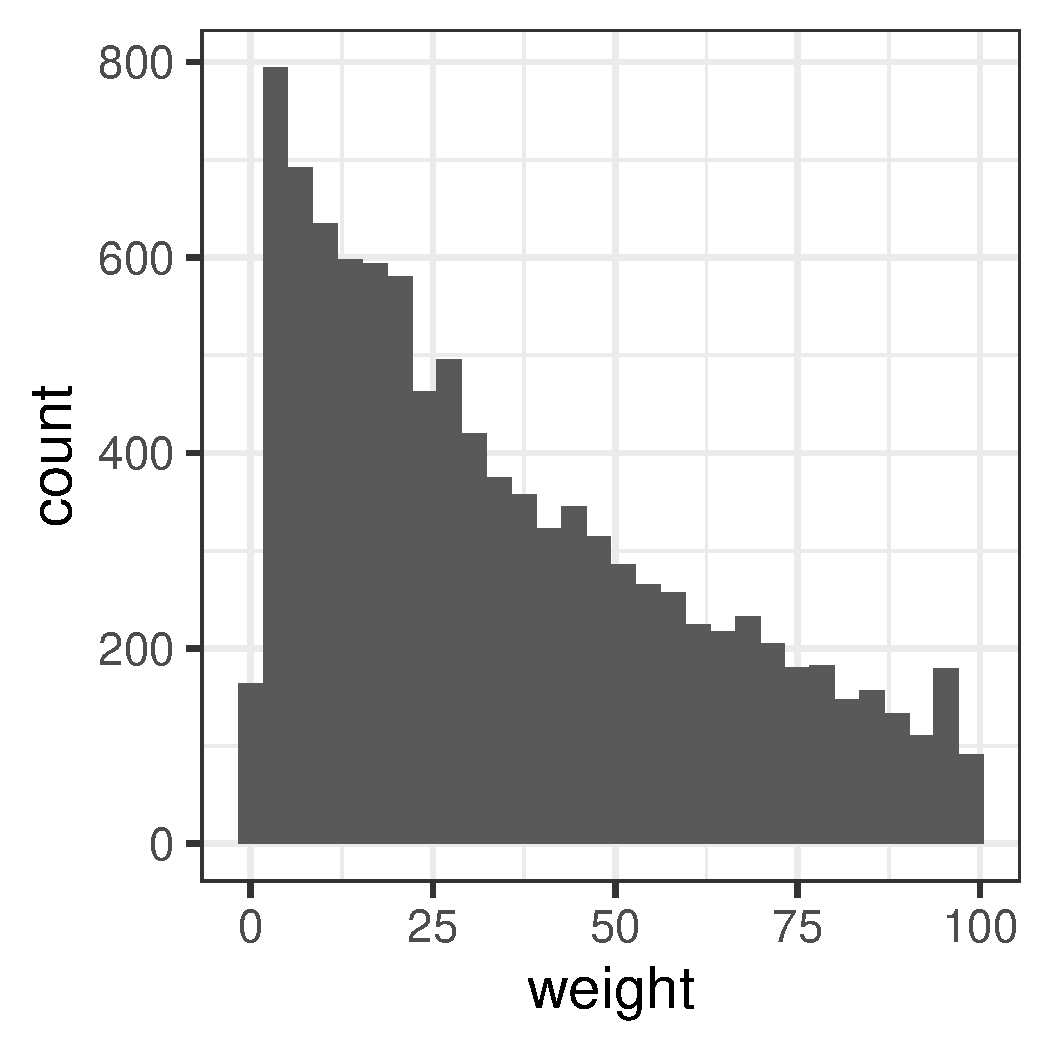
\includegraphics[width=\maxwidth]{figures/figure7regionsunnamed-chunk-19-1} 
\begin{kframe}\begin{alltt}
\hlkwd{ggsave}\hlstd{(}\hlstr{"gg1-weight.pdf"}\hlstd{,} \hlkwc{width} \hlstd{=} \hlnum{20}\hlstd{,} \hlkwc{height} \hlstd{=} \hlnum{12}\hlstd{)}
\end{alltt}


{\ttfamily\noindent\itshape\color{messagecolor}{\#\# `stat\_bin()` using `bins = 30`. Pick better value with `binwidth`.}}\end{kframe}
\end{knitrout}
\subsection{Std}

Rhat:
\begin{knitrout}
\definecolor{shadecolor}{rgb}{0.969, 0.969, 0.969}\color{fgcolor}\begin{kframe}
\begin{alltt}
\hlstd{draws} \hlkwb{<-} \hlkwd{createdraws}\hlstd{(}\hlstr{"std"}\hlstd{)}

\hlkwd{Rhat}\hlstd{(draws)}
\end{alltt}
\begin{verbatim}
## [1] 1.004977
\end{verbatim}
\end{kframe}
\end{knitrout}

Mean etc.

\begin{knitrout}
\definecolor{shadecolor}{rgb}{0.969, 0.969, 0.969}\color{fgcolor}\begin{kframe}
\begin{alltt}
\hlkwd{tail}\hlstd{(draws)}
\end{alltt}
\begin{verbatim}
##             [,1]     [,2]
## [5004,] 16.98274 13.44250
## [5005,] 16.98274 13.03193
## [5006,] 16.98274 22.11548
## [5007,] 16.98274 22.11548
## [5008,] 16.98274 22.11548
## [5009,] 16.98274 17.42381
\end{verbatim}
\begin{alltt}
\hlkwd{mean}\hlstd{(}\hlkwd{c}\hlstd{(draws[,} \hlnum{1}\hlopt{:}\hlnum{2}\hlstd{]))}
\end{alltt}
\begin{verbatim}
## [1] 16.07252
\end{verbatim}
\begin{alltt}
\hlkwd{median}\hlstd{(}\hlkwd{c}\hlstd{(draws[,} \hlnum{1}\hlopt{:}\hlnum{2}\hlstd{]))}
\end{alltt}
\begin{verbatim}
## [1] 15.22213
\end{verbatim}
\begin{alltt}
\hlkwd{sd}\hlstd{(}\hlkwd{c}\hlstd{(draws[,} \hlnum{1}\hlopt{:}\hlnum{2}\hlstd{]))}
\end{alltt}
\begin{verbatim}
## [1] 4.627666
\end{verbatim}
\begin{alltt}
\hlstd{g1} \hlkwb{<-} \hlkwd{ggplot}\hlstd{(}\hlkwd{data.frame}\hlstd{(}\hlkwc{std} \hlstd{=} \hlkwd{c}\hlstd{(draws[,} \hlnum{1}\hlopt{:}\hlnum{2}\hlstd{])),} \hlkwd{aes}\hlstd{(std))}
\hlstd{g1} \hlkwb{<-} \hlstd{g1} \hlopt{+} \hlkwd{geom_histogram}\hlstd{()} \hlopt{+} \hlkwd{theme_bw}\hlstd{(}\hlnum{28}\hlstd{)}
\hlstd{g1}
\end{alltt}


{\ttfamily\noindent\itshape\color{messagecolor}{\#\# `stat\_bin()` using `bins = 30`. Pick better value with `binwidth`.}}\end{kframe}
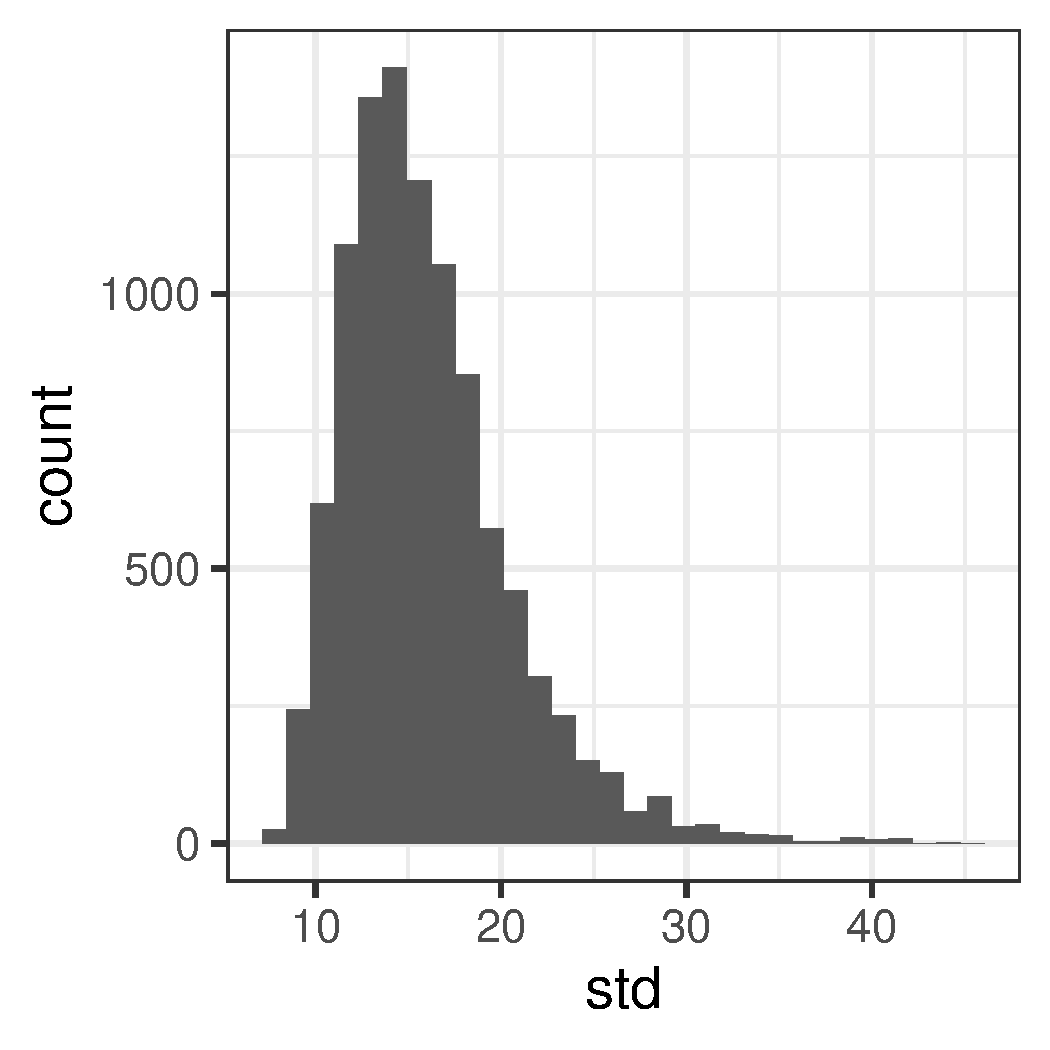
\includegraphics[width=\maxwidth]{figures/figure7regionsunnamed-chunk-21-1} 
\begin{kframe}\begin{alltt}
\hlkwd{ggsave}\hlstd{(}\hlstr{"gg1-std.pdf"}\hlstd{,} \hlkwc{width} \hlstd{=} \hlnum{20}\hlstd{,} \hlkwc{height} \hlstd{=} \hlnum{12}\hlstd{)}
\end{alltt}


{\ttfamily\noindent\itshape\color{messagecolor}{\#\# `stat\_bin()` using `bins = 30`. Pick better value with `binwidth`.}}\end{kframe}
\end{knitrout}

\end{document}
